\section {Bias Variance trade off}
The Bias variance trade off is an important part of modeling and if not done right, the model will not perform well. The model should explain the known data but also predict unseen data. A model with high variance represent the training data well, but are at risk of overfitting hence also capturing the noise in training data. On the other hand models with high bias produce simpler models and underfit their training data, therefore failing to explain the known data.

\begin{figure}[h]
	\centering
	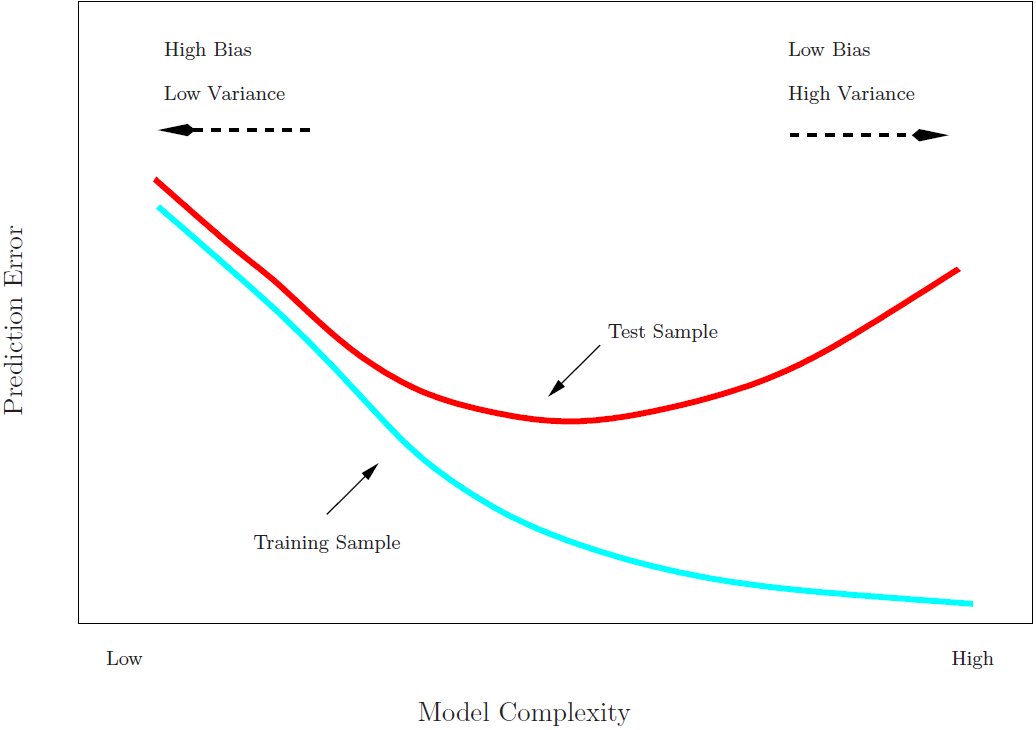
\includegraphics[width=0.5\linewidth]{crossValidation/biasVariance}
	\caption{Bias Variance trade off}
	\label{fig:biasvariance}
\end{figure}
